\graphicspath{{images/}}

\section{\thesection~Discussion}
\label{sec:discussion}

Fitness ranking from competition model fits may be better than from
logistic model fits (Will comparing stripes rankings reveal
anythin?). However, we cannot quantitatively compare fitness estimates
between plates because we are not finding global minima. Work has
begun to develop a genetic algorithm to do so. I am not convinced that
this will succeed because growth is systematically overestimated when
we move from the filled to striped plate for all of the current best
parameter solutions. This suggests an issue with the modelling
approach; below I suggest ways in which this could be improved. In
any case, qualitative cross-plate validation using order of fitness
ranking may still be better (for the competition model).

The first thing to notice about QFA data - from P15, the striped
plate, and the filled plate - is the characteristic endpoint in growth
on each plate (experiments could be designed to study variation in
timescales over regions of a plate by inoculating cultures in columns
left-to-right according to fitness). This suggests a plate-level or
region-level growth-limiting effect.
//
Could this conceivably be an experimental limitation such as the
drying out of an agar plate over time?
//
Comparison of the striped and filled data, shows that cultures grow
larger when neighbours are removed and this suggests a direct
interaction between cultures. The strongest candidates are competition
for nutrients and growth limiting signalling such as ethanol
poisoning. It is possible that other growth limiting effects may exist
and could confound any attempt to fit a model which accounts for just
one of these. It makes sense to investigate each likely effect in turn
to determine its contribution and to start by validating the
independent limit.


Spots can grow after a long time. Must be nutrients remaining or an
encroachment? I have an image for the stripes plate showing cultures
growing and believe after a very late stage. I need to check the data
images but this may just be encroachment of another culture.
\graphicspath{{images/stripes/}}
\begin{Figure}
  \centering
  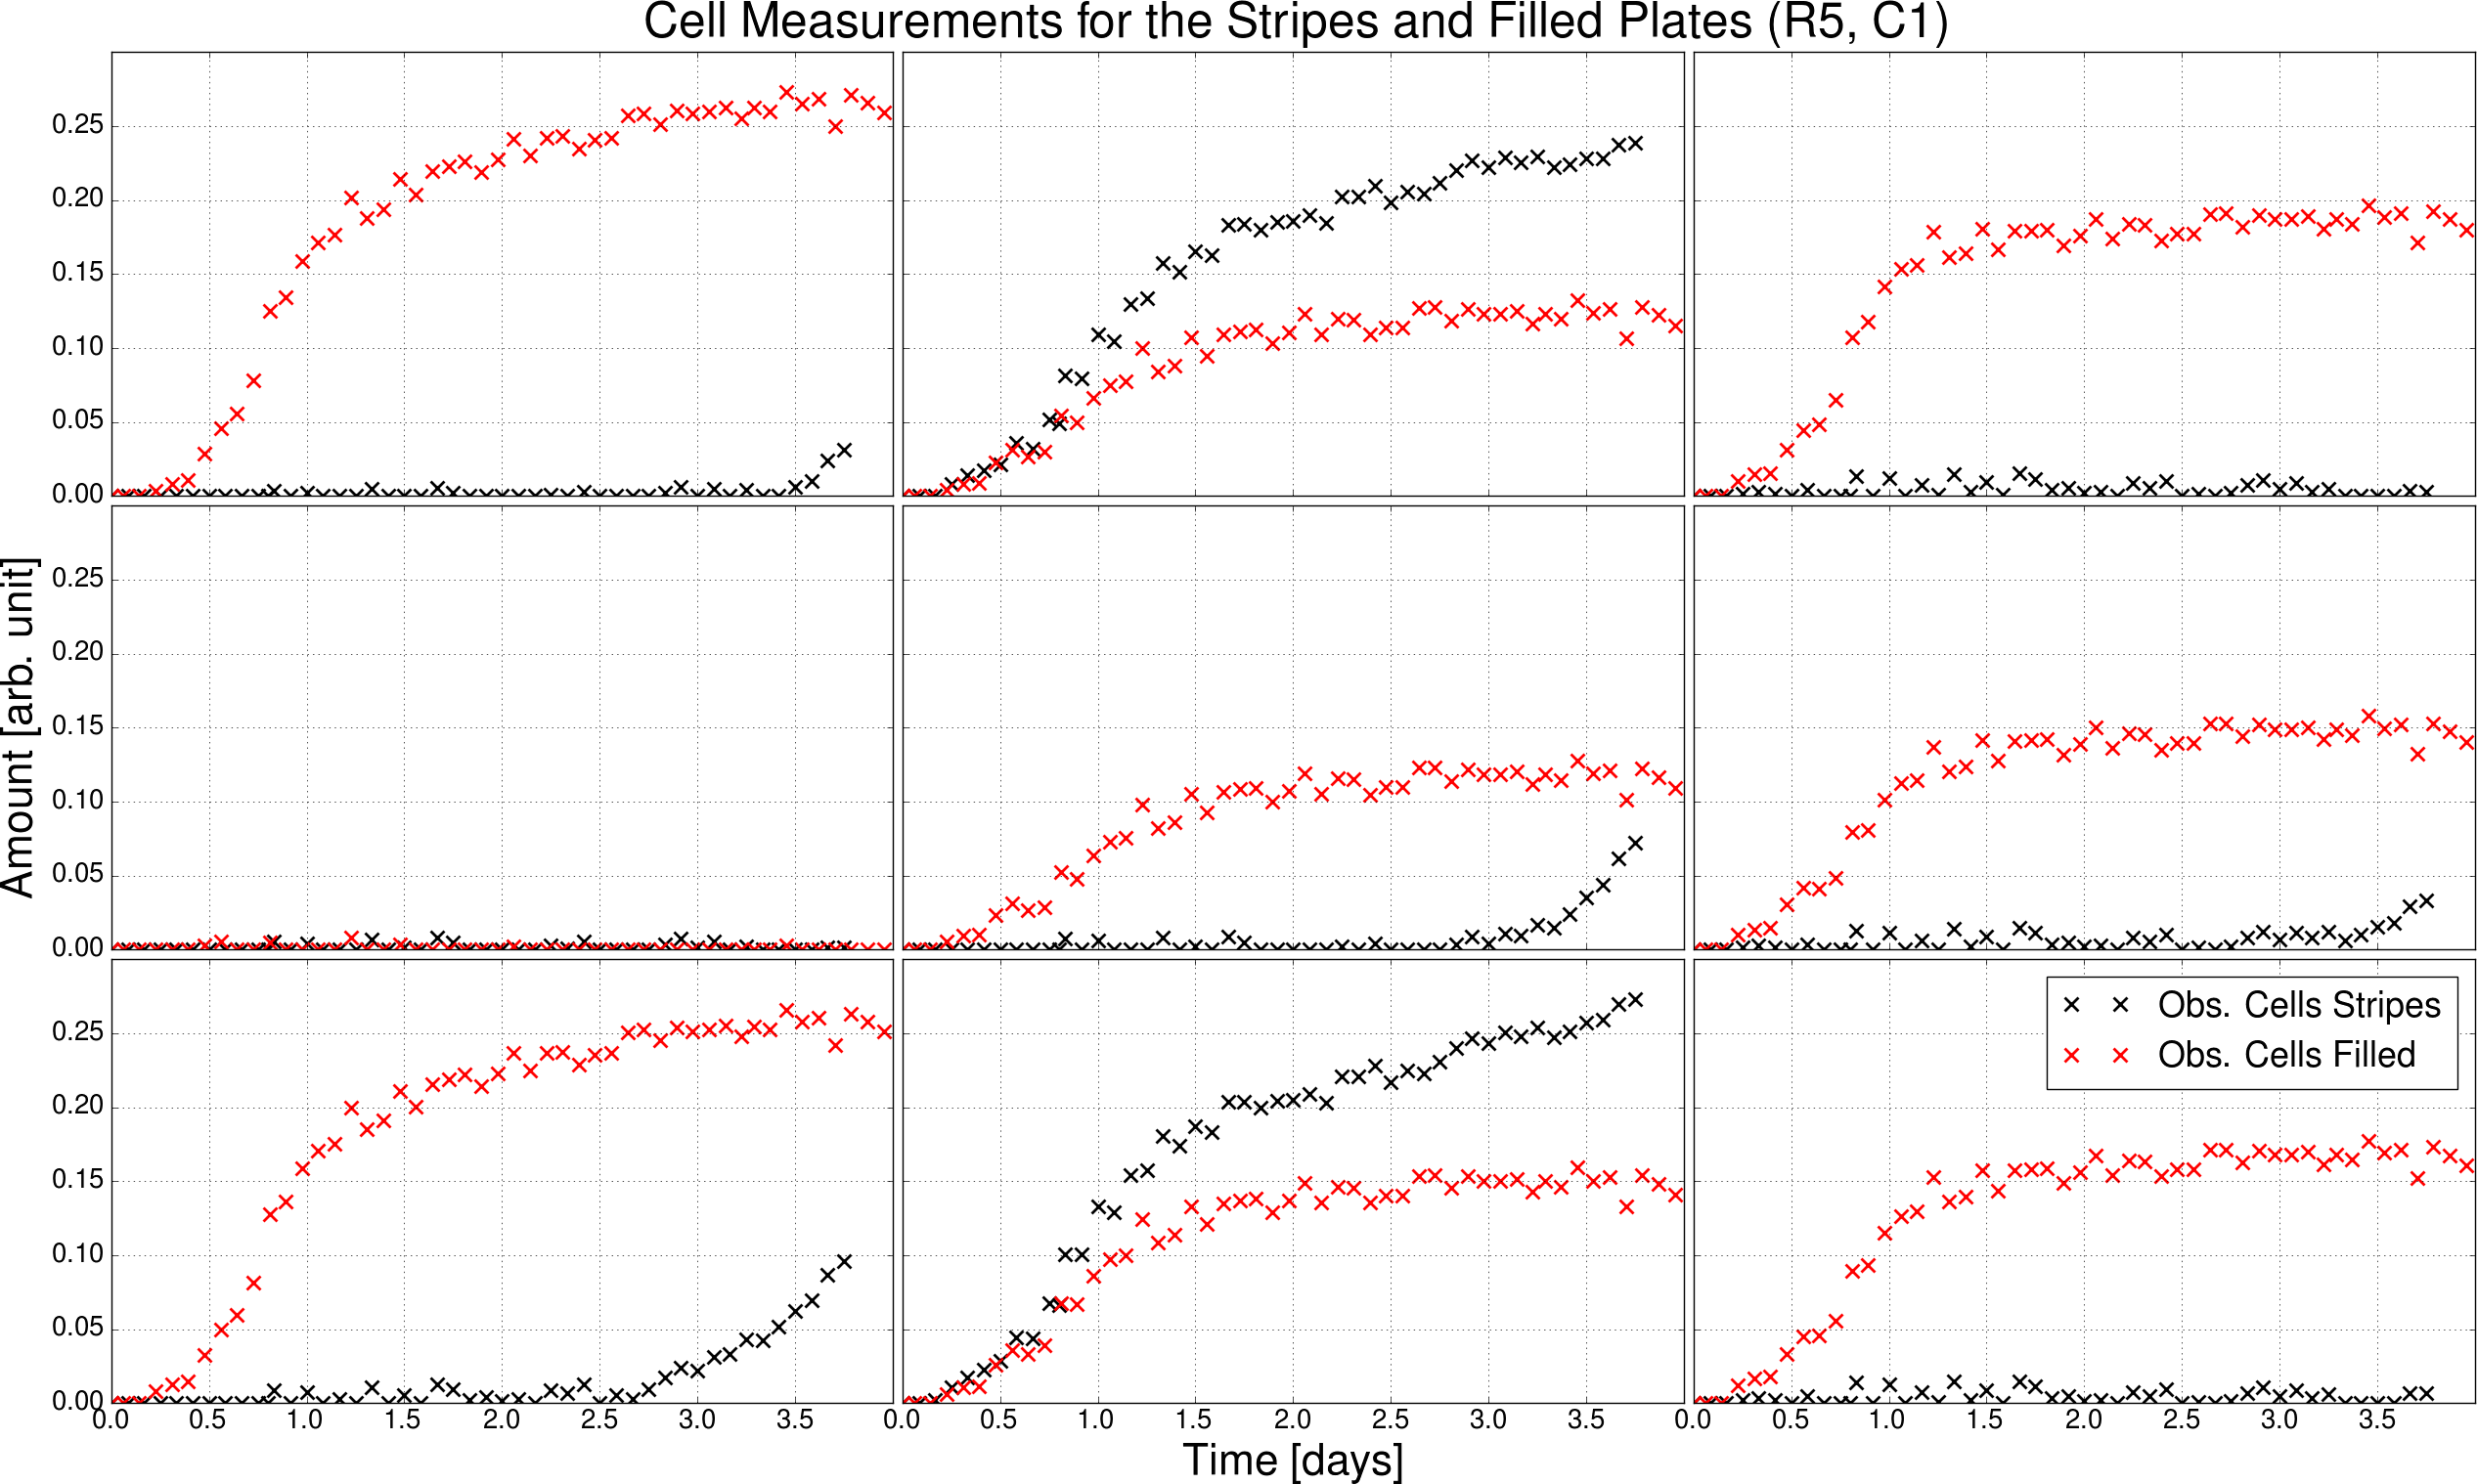
\includegraphics[width=\linewidth]{final/c_meas_r5_c1}
  \captionof{figure}{Observed cells for (R5, C1) 3x3 zone of Stripes
    and Filled plates showing (for Stripes data) slow growing cultures
    starting to grow after faster growing cultures have reached the
    stationary phase.}
  \label{fig:kn_guessing}
\end{Figure}


We have only studied data where cultures are grown in an array on
solid agar where we cannot validate the independent limit. In this
limit, our model says that nutrients can only be converted to cells
and all cultures starting with the same amount of nutrients will reach
the same final cell density. This ignores metabolism which may differ
between strains. Cell arrest could also limit growth (and this may
occur in different strains at different rates). If present,
differences in such effects could account entirely for differences in
final cell density. However, they are unlikely to be the only effect,
because this would not lead to the observed characteristic endpoint in
growth. Using one-culture spot tests (in a perti-dish on ager?) or
liquid cultures we can grow cultures independently and validate the
independent limit. A current issue with methods for estimating
fitness, is that identical strains grow differently on agar or in
liquid culture leading to different fitness rankings (cite). This
problem need not affect our validation as we can simply define a
culture to have different parameters for growth in either medium. A
greater difference may be caused by the dimensionality of the
environment. Mass action kinetics is derived for reactions in a
three-dimentsional (gas or fluid?) (Guldberg and Waage C.M. Guldberg
and P. Waage, Studies Concerning Affinity, C. M. Forhandlinger:
Videnskabs-Selskabet i Christiana (1864), 35) and this approximation
is more valid for liquid cultures than for cultures spotted onto a
surface. I suggest to study first the more ideal case of liquid
cultures and later see if the model holds for cultures grown on a
surface. If it does not, it may be necessary to use a fractal kinetics
model (I have references for this from the proposal) or, if the
reaction is diffusion limited, consider a more detailed model of
nutrient diffusion.

// Model equations for metabolism.//

Our model splits the agar into a grid with volume discretised per
culture. In the stripes validation, we overestimate the effect of
diffusion when neighbouring cultures are removed. I believe that we
are not accurately capturing the point at which growth becomes
diffusion limited and that nutrients are well approximated as being
evenly distributed withing the spatial scales that we model. A
diffusion equation model could capture the local distribution of
nutrients around a culture when the stationary phase is reached.  Reo
and Korolev (2014) use the diffusion equation (and Neumann and
Dirichlet boundary conditions) to simulate nutrient dependent growth
of a single bacterial culture on a pertri dish in two-dimensions. They
create a sink for nutrients from culture growth and equate the flux of
nutrients through the culture area with the rate of increase in
culture size. They model culture area as varying and keep culture
density constant. We may instead keep culture area constant, allow
culture density to vary, and use our mass action kinetic model (eq
no.) for the nutrient sink and culture growth. Simulating or fitting
this model could help us learn more about diffusion in QFA
experiments.  It is probably computationally unfeasible to use such a
detailed model to fit a whole plate. However, if necessary, it may be
possible to use a finer grid to increase compartmentalisation of
nutrients to capture spatial heterogeneity in the distribution of
nutrients around a culture and the effect of diffusion limited
growth. This could extend the validity of the competition model over a
larger range of variability in culture growth rates (for instance when
some cultures are left empty and others are very fast growing.)

It would also be useful to determine experimentally how nutrients are
distributed throughout the agar at the stationary phase. Gaps could be
left in an array of cultures and only inoculated once the stationary
phase is reached. If they grow then nutrients remain. (Sill require
simulations to see distribution across depth). This could be extended
by growing a single column of identical strains and, after the
stationary stage has been reached, inoculating identical strains on
the same plate at different distances from the row.

//Talk about an improvement to the imaginary neighbour model.//

Nutrients (sugars, nitrogen, etc.) in QFQ agars are of a standard
composition, designed to reduce the excess of any single nutrient
(check QFA paper and cite). ((background) What is the nutrient?
Nitrogen is only used to build molecules for new cells, whereas sugars
are also used for metabolism.) For modelling nutrient limited growth,
especially across plates, it would be useful to know the identity of
the limiting nutrient and ensure that it is always the same. We could
achieve this using a different formula of agar.

The design of the stripes validation experiment could be
improved. Rather than filling gaps with cultures not present on the
stripes plate, and for which we have no b estimates, we could fill
with repeats of the cultures already present on the stripes
plate. (I'm not sure it makes any difference actually whether we
validate from one direction to the other). It would also have been
helpful to have repeats to study differences in COV between the
competition and independent models. In order to make sure that
competition effects were present in data, we made a drastic change
between the stripes and filled plates. This provides a stern
validation. The model assumes that competition effects are present
whenever there is a difference in final cell amounts between
cultures. We could have first validated the model against a smaller
change, by varying between slower and faster growing cultures rather
that none and very strong growing cultures. If the model works well
between such plates it may work well for the majority of QFA
experiments which typically have smaller differences between cultures
than the data we study. If we did want to test the in an extreme case
we could have inoculated fast growing cultures next certain strains
and not others to try to induce a change in ranking for which the
competition model might compensate better than the logistic model.

//Signalling//

If we find that competition for nutrients is not a significant effect,
for instance if growth becomes diffusion limited before nutrients from
neighbours can be accessed, then we could instead model signalling by
ethanol as the interaction effect. This may be modelled similarly to
how we are already modelling nutrient diffusion.

//Signalling equation//

If there is any combination of competition, metabolism, signalling, or
arrest contributing significantly to differences in the growth of
cultures and the interaction between neighbours then it will be
difficult to separate them when fitting a model to data. We may have
to develop ways to calibrate effects in isolation (e.g. by
adding/measuring ethanol?) and use this information when fitting to
high-throughput data.

It is quicker to fit to small zones of a plate but as these have a
larger proportion of edge cultures boundary conditions become
important. In current data (e.g. P15), different cultures surround the
edge and this makes accurate fitting difficult. As a result we must
work with larger zones that take longer to analyse. We could surround
small 3x3 and 4x4 zones with an empty ring and only need to consider
net flux of nutrients across the boundary and not local variation due
to different cultures surrounding the zone. We could also surround
with the same, low-variance, strain to reduce net flux.
% (Would it be better not to use a temperature dependent strain?)

//Stochastic effects.//

Unpublished work by Hermann and Lawless has investigated heterogeneity
between cell lines within single QFA spots. They have found that a
single or small number of extremely fast growing cell-lines come to
dominate the population of a single culture. The implication is that
cultures with a lower starting cell densities are likely to have
greater variance between repeats. We could use higher starting cell
concentrations to reduce this variance but then we study less of the
growth phase. It may be possible to reduce heterogenetity by inoculating
from the exponential growth phase rather than the stationary phase and
still study full growth curves. (Unless mean population growth
constant is being studied...) Staring cell densities should ideally be
as close to the lowest resolvable level as possible.

//Ways to measure \(C_{0}\)// There is a confounding effect between
initial cell density and b value with may justify using initial cell
densities slightly above the minimum detectable level. Hetoregeneity
within cultures is an issue again here and cell density would
effectively be lower than the measured value, e.g., if most inoculated
cells are dead or slow growing.

To fit growth curves more accurately QFA has begun using the
generalised logistic model (cite). Fitness estimates (MDR*MDP or MDR?)
from this model have higher coefficient of variation than those from
either the standard logistic or competition model. (accuracy and
precision? Could for instance a step function be less variable than
the standard logistic model?)  Although the fits to data are
qualitatively worse, it may be advisable to revert to the standard
logistic model.


The logistic model requires different K parameters (\(N_{0}\) for
log. eq.) to be fit for each culture. The competition model shares
information about \(N_{0}\) between cultures and therefore has 383
fewer parameters for a full plate (Could this also explain the higher
variance for the fastest growers?). For the slowest growing cultures,
noise is more dominant and there is a confounding effect between r and
K. To deal with this, the QFA R package uses heuristic checks. In the
case of \textit{est1\(\Delta\)}, this has led to a dramatic
disagreement in estimated fitness with the competition model. The
estimate from (which model)? agrees better with existing biological
knowledge (/independent spot experiments?). (Is the competition model
then useful?)

//QFA R is fixing \(C_{0}\) rather than fitting (I used a grid))//

//Improvement to imaginary neighbour guessing//


%%% Local Variables:
%%% mode: latex
%%% TeX-master: "report"
%%% End:
